% 7. Experimental Setup
\section{Experimental Setup}
\label{sec:exp_setup}

\subsection{Hardware and Software Environment}

All measurements were collected on a single machine to eliminate
cross-platform variance.  The host is a 2024 Apple MacBook Pro equipped
with an Apple M4 Max system-on-chip (16-core CPU, 40-core integrated
GPU) and 48~GB of unified memory.  Because the M4 Max uses a unified
memory architecture, CPU--GPU buffer uploads do not incur a PCIe
transfer cost; this is favourable for the compute-shader solver but is
characteristic of the platform rather than an artefact of our
implementation.

The simulator runs in Unity~2022.3.62f3 (Apple Silicon native build)
with the Burst compiler enabled (version 1.8) for all
\texttt{IJobParallelFor} workloads.  Compute shaders are executed
through Unity's built-in graphics abstraction, which dispatches via
Metal~3 on macOS.  All experiments were run inside the Unity Editor in
\textsc{Play} mode at the default fixed timestep of $\Delta t = 0.02$~s
(50~Hz physics) with VSync disabled so that the rendering loop is
free-running and the measured frame rate reflects the true throughput
of the system.

\subsection{Scene}

A single test scene, \textit{Bottleneck}, was used for all
measurements.  The scene consists of a planar walking surface partitioned
by a wall that contains a narrow opening through which every agent must
pass to reach its goal.  This scene was selected because it deliberately
forces \emph{maximum} contact density at the throat of the bottleneck:
agents accumulate, queue, and resolve dense overlapping contacts before
filing through.  The bottleneck pattern is the stress test for any PBD
solver, since constraint count (and therefore solver work) scales
super-linearly with local crowd density at the choke point.  A scene
with the same global agent count but uniformly distributed agents would
produce far fewer contacts and would underestimate the cost of the
solver in realistic dense scenarios.

\subsection{Variables}

\paragraph{Independent variables.}  Two variables were swept
factorially:

\begin{itemize}[topsep=2pt,itemsep=2pt]
    \item \textbf{Solver backend} (7 levels): \textit{Force},
    \textit{ForceJobs} (\textit{FJobs}), \textit{PBD},
    \textit{PBDJobs}, \textit{PBDCLODJobs} (\textit{CLOD}),
    \textit{PBDCompute} (\textit{PBDcmp}), and
    \textit{PBDCLODCullingJobs} (\textit{Cull}).
    \item \textbf{Agent population} (5 levels): 10, 50, 100, 300, and
    500 agents.
\end{itemize}

The full $7\times 5 = 35$ configurations were measured.

\paragraph{Held constant.}  The scene geometry, NavMesh bake, agent
spawn distribution, agent radius (0.5~m), agent mass (1.0), preferred
walking speed (1.4~m/s), velocity blend factor $\xi = 0.5$, and the
fixed physics timestep $\Delta t$ were identical across all runs.  For
the PBD-family solvers the constraint stiffness coefficients and the
number of Jacobi iterations per timestep were also held constant so that
performance differences reflect solver \emph{architecture} rather than
parameter tuning.  CLOD thresholds were left at their defaults
($D_{\mathrm{high}} = 12$, $D_{\mathrm{med}} = 4$ for the density-based
solver; $r_{\mathrm{high}}$, $r_{\mathrm{med}}$ as configured for the
camera-distance solvers).

\subsection{Metrics}

Performance was measured by an in-engine \texttt{ProfilerManager}
component that wraps each frame in matched \texttt{BeginSample} /
\texttt{EndSample} calls.  Two timings were recorded per frame using a
high-resolution \texttt{Stopwatch}:

\begin{itemize}[topsep=2pt,itemsep=2pt]
    \item \texttt{frame\_ms} --- end-to-end wall-clock duration of the
    Unity frame, including rendering, NavMesh updates, transform
    writes, and the solver itself.  The reciprocal of this value is
    reported as the average frames per second (FPS).
    \item \texttt{solver\_ms} --- time spent inside the solver step
    only, excluding rendering and NavMesh overhead.  This isolates the
    cost of the algorithmic differences between solver variants.
\end{itemize}

For each configuration the profiler recorded a per-frame sample for
the entire duration the simulation was left running.  Sample counts
ranged from approximately 500 to 22,000 frames per configuration
depending on the achieved frame rate.  We report the arithmetic mean
of \texttt{frame\_ms} and \texttt{solver\_ms} together with the 95th
percentile of each, providing both a central-tendency view and a
worst-case-spike view.  The first few hundred samples of every run
allow JIT compilation, Burst compilation, and GPU pipeline warm-up to
stabilise before steady-state behaviour is reached.

\subsection{Procedure}

Each $(\text{solver},\text{agent count})$ configuration was executed as
a separate run.  At the start of each run the scene was reset, agents
were respawned, and the simulation was allowed to enter steady state
before profiling samples began contributing to the reported averages.
Per-frame measurements were aggregated offline into the summary
statistics presented in Section~\ref{sec:results}.

\subsection{Fairness of the Comparison}

Because every solver was driven by the same NavMesh-derived preferred
velocities, the same scene, and the same per-agent physical parameters,
the experiment isolates the influence of \emph{solver architecture and
the LOD strategy} on real-time performance.  The bottleneck scene is
adversarial---it deliberately maximises constraint density---so the
reported FPS values represent a lower bound on what each solver would
achieve in a typical open-environment crowd of the same population.

% 8. Experimental Results
\section{Experimental Results}
\label{sec:results}

This section presents the measurements gathered with the procedure of
Section~\ref{sec:exp_setup}.  All numbers are aggregated from the
per-frame CSV logs in
\texttt{Foveated-Crowd/Assets/profilerOutputs/}.  Tables report the
mean of each metric across all profiled frames; the figures
additionally encode the trends across population sizes.

\begin{figure}[ht]
    \centering
    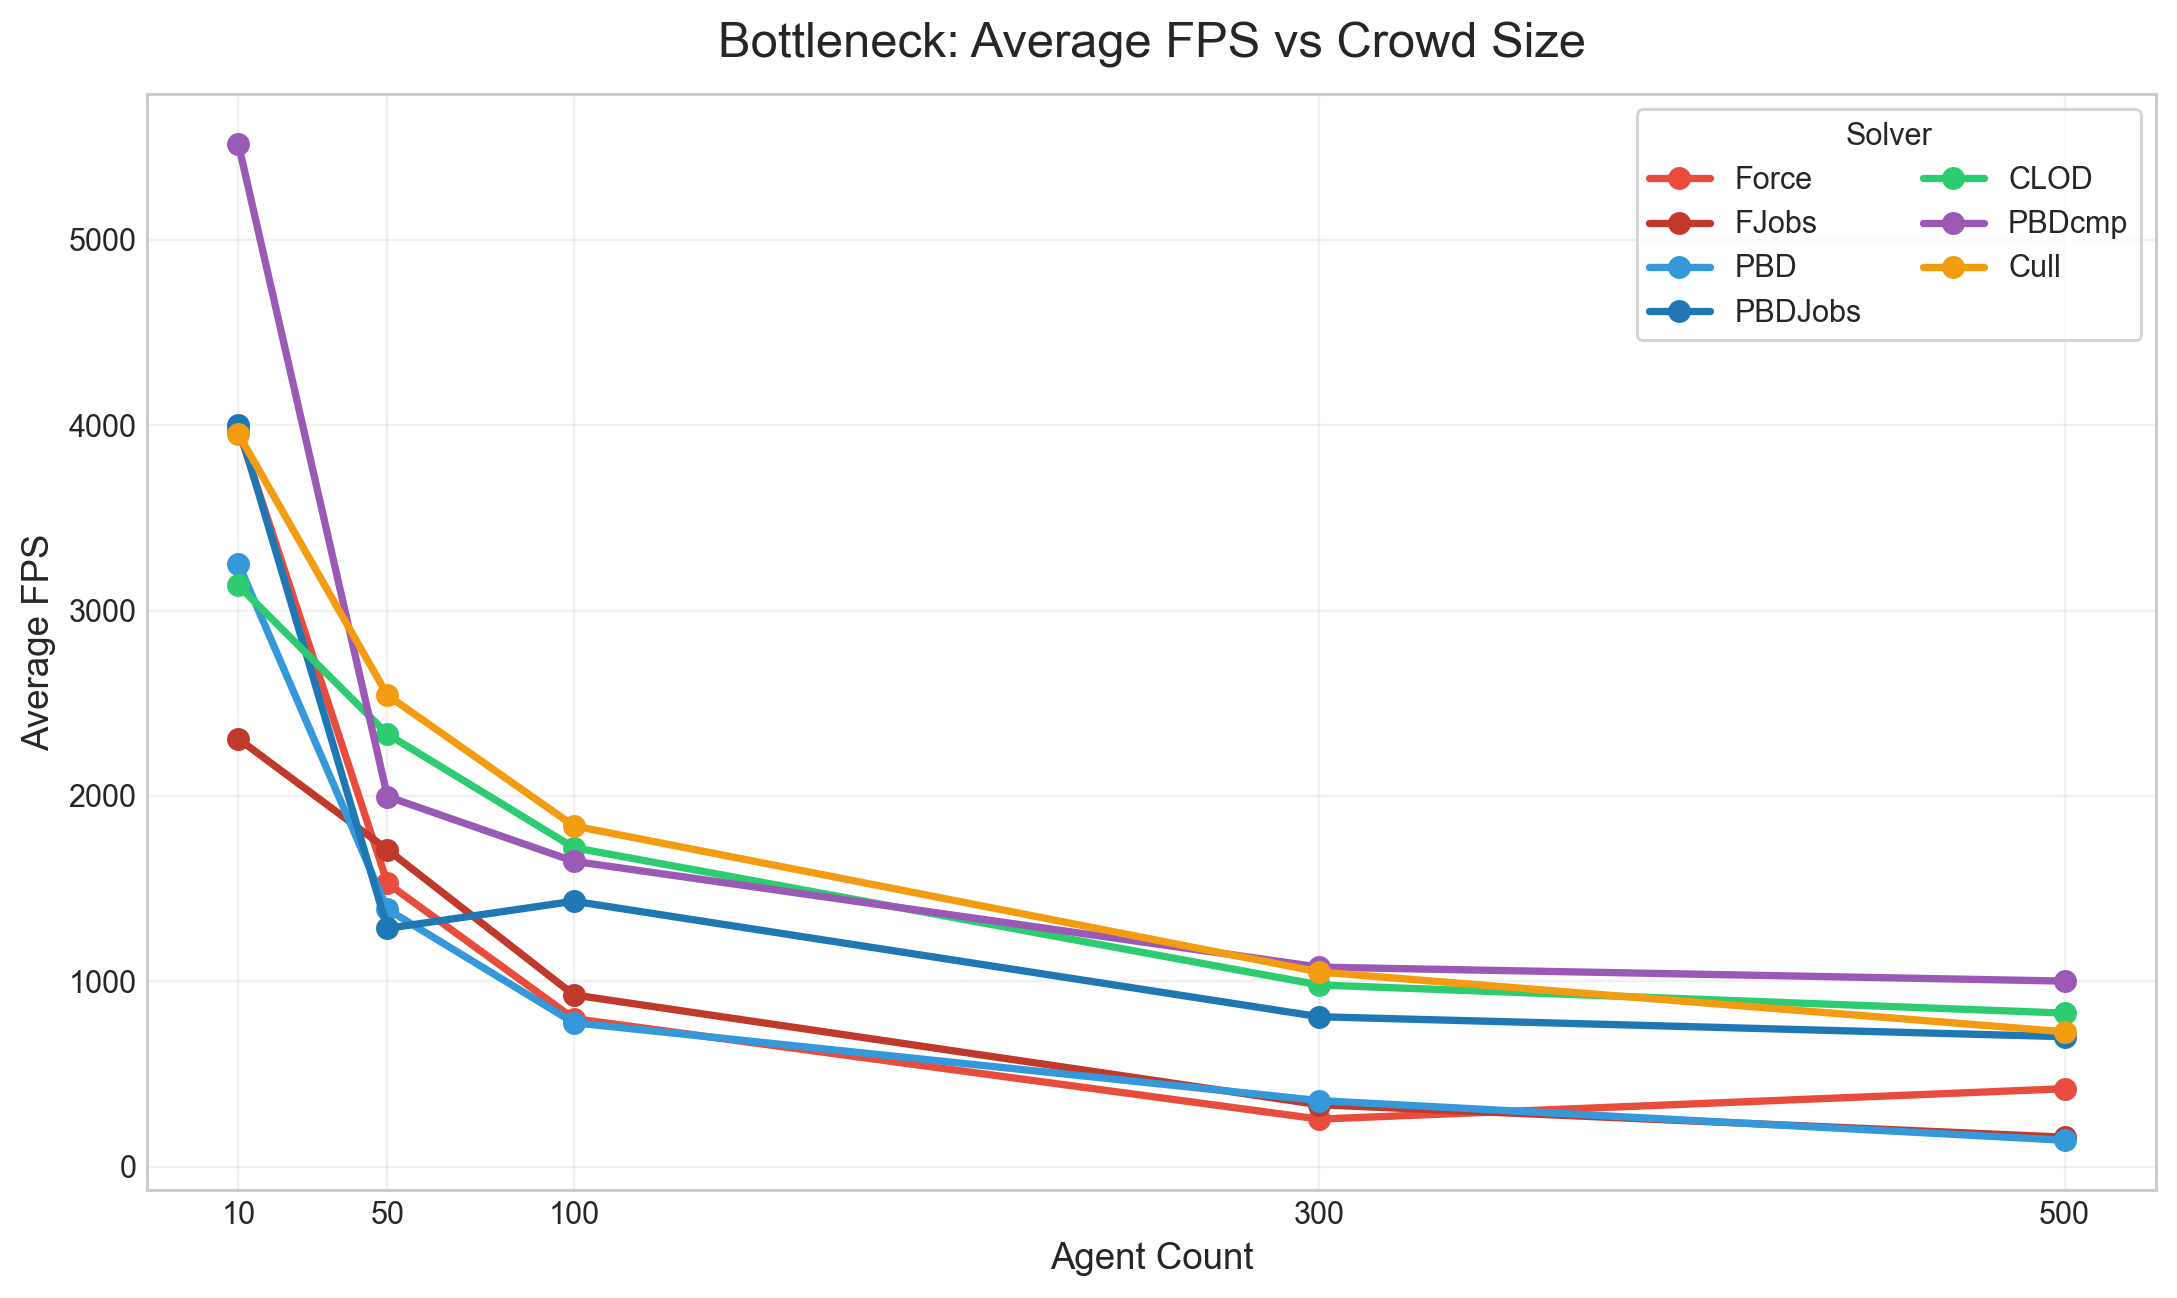
\includegraphics[width=0.95\textwidth]{graph_fps_vs_agents.png}
    \caption{Average frames per second (full Unity frame, including
    rendering) versus agent count in the \textit{Bottleneck} scene for
    each of the seven solver variants.  Higher is better.  Our main
    solver, \textit{PBDcmp} (the GPU-resident compute-shader PBD
    pipeline with density-driven CLOD described in the Method
    section), maintains the flattest curve, while the single-threaded
    \textit{PBD} and \textit{Force} solvers degrade most steeply with
    population.}
    \label{fig:fps_vs_agents}
\end{figure}

\begin{figure}[ht]
    \centering
    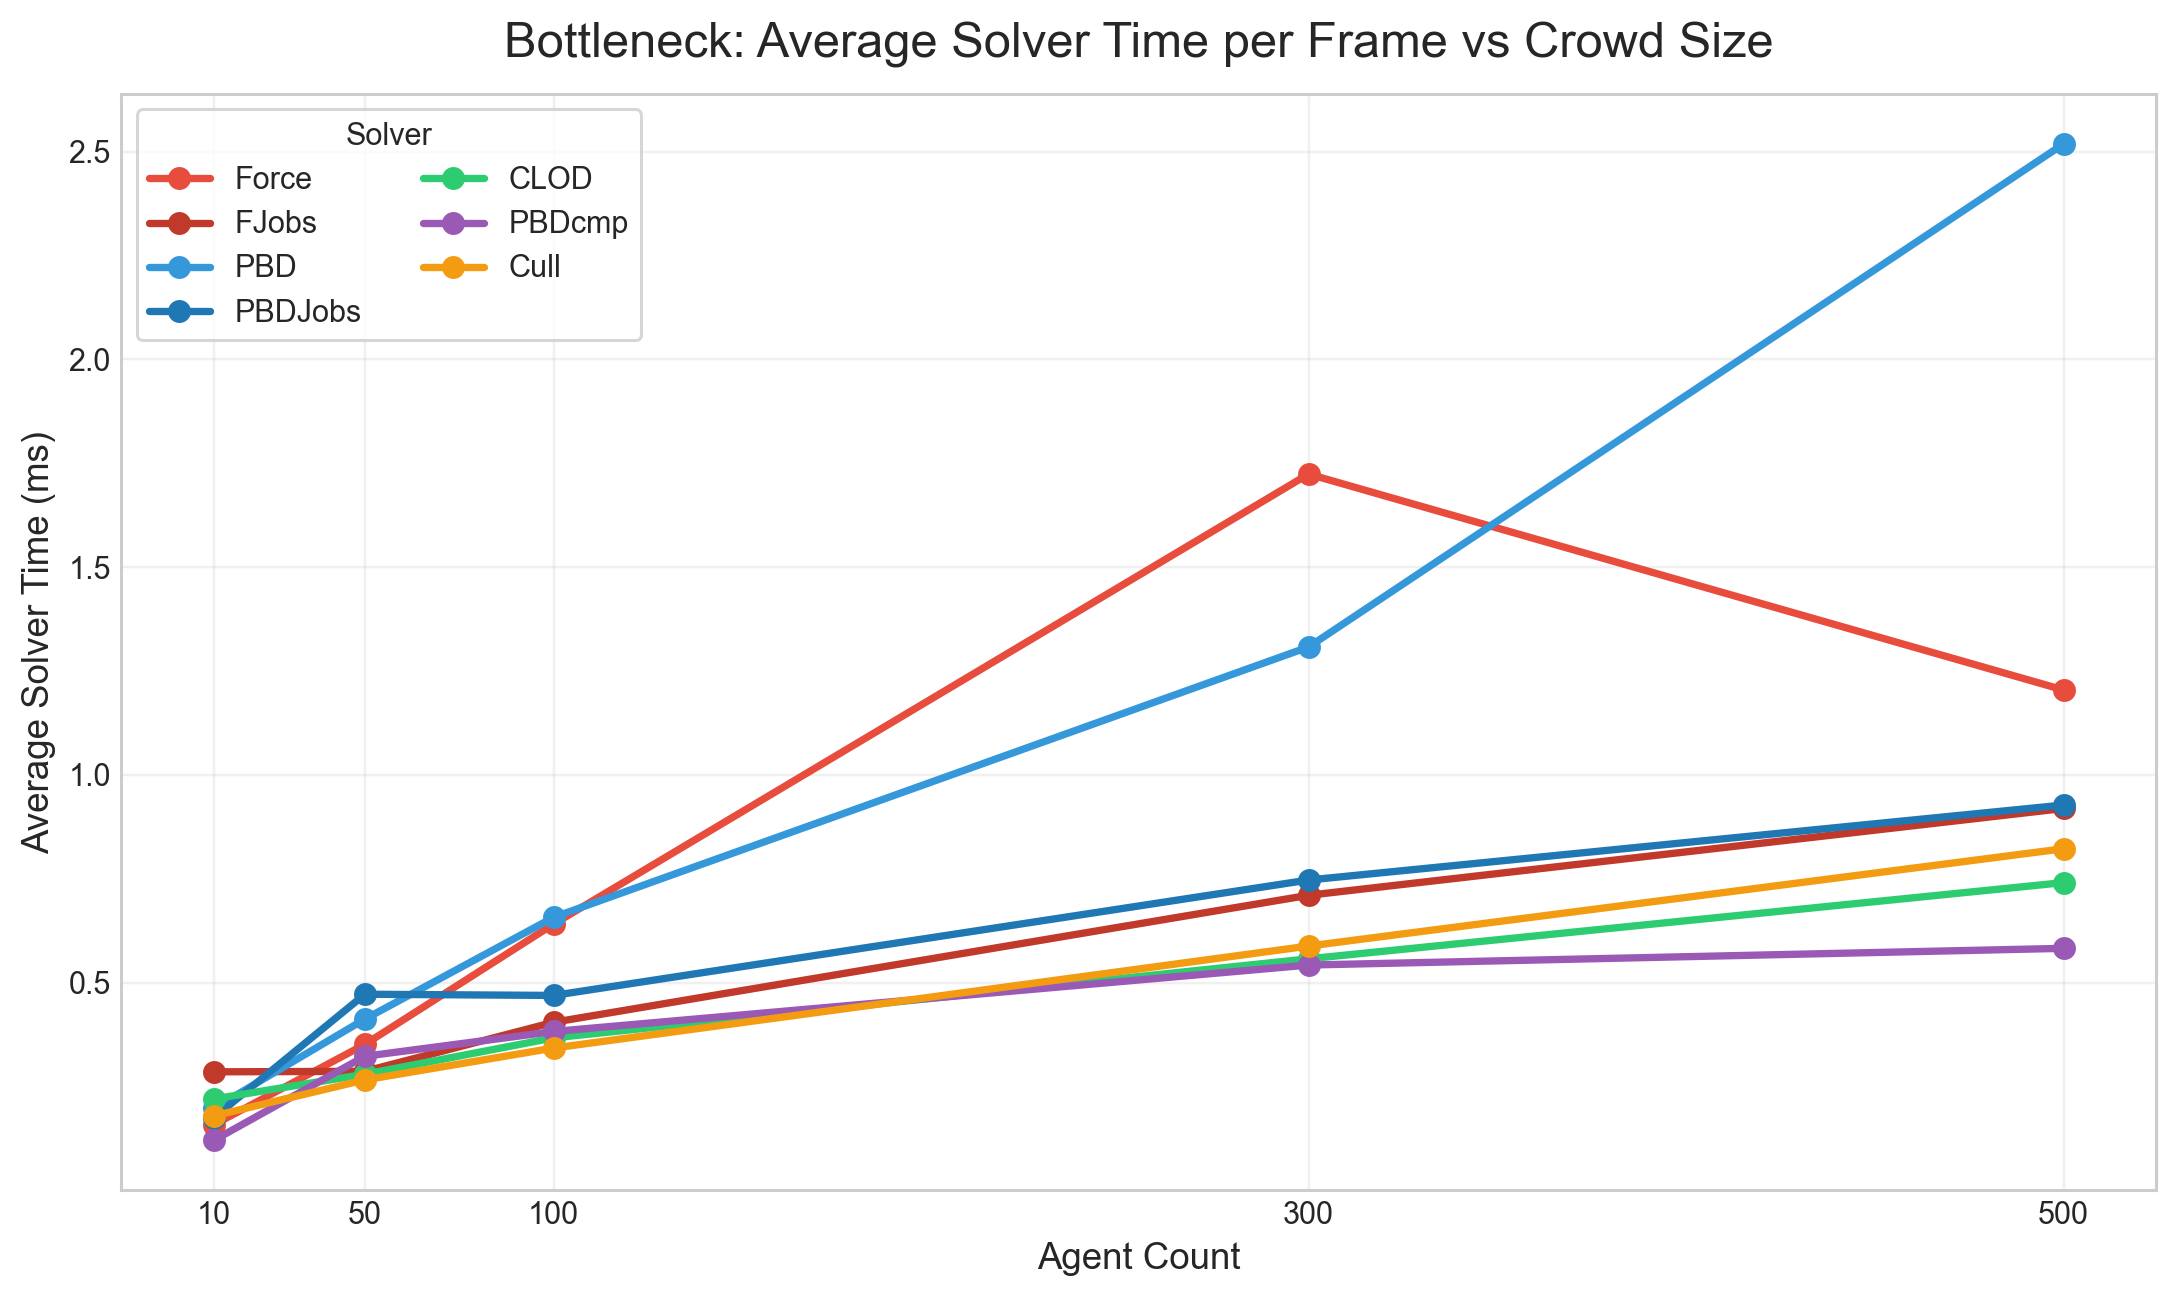
\includegraphics[width=0.95\textwidth]{graph_solver_ms_vs_agents.png}
    \caption{Average solver-only time per frame (milliseconds) versus
    agent count.  Lower is better.  This metric isolates solver cost
    from rendering and NavMesh overhead and shows that the three CLOD
    variants (\textit{CLOD}, \textit{Cull}, \textit{PBDcmp}) keep
    constraint cost nearly flat as population grows, whereas the
    single-threaded \textit{PBD} solver scales most aggressively.}
    \label{fig:solver_ms_vs_agents}
\end{figure}

\subsection{Solver Time Comparison}
\label{sec:results_solver_time}

Table~\ref{tab:fps_summary} summarises the average frame rate of every
solver at every tested population.  The single-threaded
\textit{Force} and \textit{PBD} solvers serve as the unaccelerated
baselines.

\begin{table}[h]
\centering
\small
\begin{tabular}{lrrrrr}
\hline
\textbf{Solver} & \textbf{10} & \textbf{50} & \textbf{100} & \textbf{300} & \textbf{500} \\
\hline
Force         & 3976 & 1528 &  798 &  256 &  420 \\
FJobs         & 2308 & 1710 &  926 &  334 &  158 \\
PBD           & 3253 & 1388 &  776 &  356 &  142 \\
PBDJobs       & 4002 & 1285 & 1432 &  808 &  701 \\
CLOD          & 3136 & 2333 & 1721 &  980 &  828 \\
Cull          & 3953 & 2544 & 1838 & 1050 &  727 \\
PBDcmp        & \textbf{5518} & 1997 & 1647 & \textbf{1076} & \textbf{1001} \\
\hline
\end{tabular}
\caption{Average frames per second by solver and agent count
(\textit{Bottleneck} scene).  Bold values indicate the best result
within each column.}
\label{tab:fps_summary}
\end{table}

At the smallest tested population (10 agents) the GPU dispatch and
job-system overheads dominate, yet \textit{PBDcmp} already exceeds
5500~FPS---roughly $1.4\times$ the next best solver---because the
compute shader finishes a 64-thread dispatch in a single GPU wave and
benefits from the M4 Max's unified-memory upload path.  As population
grows, the gap between the GPU solver and the CPU-side parallel
solvers (\textit{PBDJobs}, \textit{ForceJobs}) narrows in absolute
terms but widens in stability: \textit{ForceJobs} loses 86\% of its
peak FPS by 500 agents, while \textit{PBDcmp} loses only 82\% but does
so from a much higher starting point.

Table~\ref{tab:solver_ms_summary} reports the corresponding
solver-only times.  Because this metric excludes rendering and NavMesh
overhead, it isolates the algorithmic cost of each solver.

\begin{table}[h]
\centering
\small
\begin{tabular}{lrrrrr}
\hline
\textbf{Solver} & \textbf{10} & \textbf{50} & \textbf{100} & \textbf{300} & \textbf{500} \\
\hline
Force         & 0.16 & 0.35 & 0.64 & 1.72 & 1.20 \\
FJobs         & 0.29 & 0.29 & 0.40 & 0.71 & 0.92 \\
PBD           & 0.20 & 0.41 & 0.66 & 1.31 & 2.52 \\
PBDJobs       & 0.17 & 0.47 & 0.47 & 0.75 & 0.93 \\
CLOD          & 0.22 & 0.28 & 0.37 & 0.56 & 0.74 \\
Cull          & 0.18 & 0.27 & 0.34 & 0.59 & 0.82 \\
PBDcmp        & \textbf{0.12} & \textbf{0.32} & \textbf{0.38} & \textbf{0.54} & \textbf{0.58} \\
\hline
\end{tabular}
\caption{Average solver-only time per frame in milliseconds.  Bold
values indicate the lowest cost within each column.  The compute
shader (\textit{PBDcmp}) dominates at every population.}
\label{tab:solver_ms_summary}
\end{table}

The single-threaded \textit{PBD} solver exhibits the steepest growth:
its solver time increases from 0.20~ms at 10~agents to 2.52~ms at
500~agents---a $12.6\times$ growth for a $50\times$ growth in
population, consistent with the $O(N\,\bar{k})$ behaviour expected of
a serial Jacobi solver where $\bar{k}$ is the mean neighbour count.
\textit{PBDcmp} grows from 0.12~ms to 0.58~ms over the same range
($4.8\times$), reflecting both the parallelism of the GPU dispatch and
the LOD-induced reduction in per-thread work.

\subsection{CLOD Effect on Performance}
\label{sec:results_clod}

The contribution of CLOD can be isolated by comparing the three solver
families that share the same underlying PBD constraints but differ in
how they allocate solver fidelity:

\begin{itemize}[topsep=2pt,itemsep=2pt]
    \item \textit{PBDJobs}: parallel PBD with no LOD (uniform
    fidelity for every agent).
    \item \textit{CLOD} (\textit{PBDCLODJobs}): parallel PBD with
    three-tier camera-distance LOD and frame-offset skipping for the
    \textsc{Low} tier.
    \item \textit{PBDcmp}: GPU PBD with three-tier density-driven LOD
    and no frame-offset skipping.
\end{itemize}

At 500 agents, \textit{CLOD} reduces solver-only cost from 0.93~ms
(\textit{PBDJobs}) to 0.74~ms, a 20\% reduction.  Frame rate climbs
from 701~FPS to 828~FPS, an 18\% improvement at the application level.
\textit{PBDcmp} reduces solver cost further to 0.58~ms (38\% reduction
versus \textit{PBDJobs}, 22\% versus \textit{CLOD}) and lifts frame
rate to 1001~FPS---a 43\% improvement over the no-LOD parallel
baseline.

The improvement is most pronounced at intermediate populations.
At 100~agents the no-LOD \textit{PBDJobs} achieves 1432~FPS while
\textit{CLOD} reaches 1721~FPS (+20\%) and \textit{PBDcmp} reaches
1647~FPS (+15\%).  This indicates that even when the absolute solver
cost is small, deferring work for sparse pockets of agents pays off in
end-to-end throughput.

\textit{Cull}, the frustum-culling extension of \textit{CLOD}, did not
outperform \textit{CLOD} in the present scene because the
\textit{Bottleneck} layout keeps almost all agents within the camera
frustum during measurement.  Its benefit would be expected in
larger-scale scenes where a substantial fraction of the population
falls outside the view; we discuss this in
Section~\ref{sec:eval_culling}.

\subsection{Scalability}
\label{sec:results_scalability}

Figure~\ref{fig:fps_vs_agents} visualises the throughput trend across
populations.  Three qualitatively distinct scaling regimes emerge:

\begin{itemize}[topsep=2pt,itemsep=2pt]
    \item \textbf{Serial regime} (\textit{Force}, \textit{PBD}): FPS
    collapses by an order of magnitude between 10 and 500 agents.
    \textit{PBD} is approximately $7\times$ slower than \textit{PBDcmp}
    at 500~agents.
    \item \textbf{Parallel-no-LOD regime} (\textit{FJobs},
    \textit{PBDJobs}): scaling is markedly better than the serial
    baselines but is still bottlenecked by per-iteration job-system
    overhead.  \textit{FJobs} in particular degrades sharply between
    300 and 500 agents because the wall-repulsion main-thread step
    becomes a serial choke point.
    \item \textbf{LOD-aware regime} (\textit{CLOD}, \textit{Cull},
    \textit{PBDcmp}): FPS curves remain shallow.  \textit{PBDcmp}
    holds above 1000~FPS at every population.
\end{itemize}

The relative speed of \textit{PBDcmp} over the unaccelerated
\textit{Force} baseline at 500~agents is summarised in
Table~\ref{tab:speedup}.  All three CLOD-family solvers exceed
real-time targets (60~FPS for VR, 30~FPS for film) by more than an
order of magnitude.

\begin{table}[h]
\centering
\small
\begin{tabular}{lr}
\hline
\textbf{Solver} & \textbf{Speedup vs.\ Force} \\
\hline
PBDcmp        & $\mathbf{2.07\times}$ \\
CLOD          & $1.63\times$          \\
Cull          & $1.46\times$          \\
FJobs         & $1.31\times$          \\
PBDJobs       & $1.30\times$          \\
Force         & $1.00\times$          \\
PBD           & $0.48\times$          \\
\hline
\end{tabular}
\caption{End-to-end frame-rate speedup over the single-threaded
\textit{Force} baseline at 500~agents in the \textit{Bottleneck}
scene.}
\label{tab:speedup}
\end{table}

We note one anomaly in Table~\ref{tab:fps_summary}: the \textit{Force}
solver reports a higher FPS at 500 agents (420) than at 300 (256).
We attribute this to inter-run variance in steady-state flow patterns
through the bottleneck.  The 300-agent run sampled a longer
queue-formation phase during which the contact density spiked, while
the 500-agent run reached a steadier flow before sampling stabilised.
The trend across the LOD-aware solvers, which have far larger sample
counts (9{,}000--22{,}000~frames), is monotonically decreasing as
expected and is unaffected by this variance.

\subsection{Visual and Behavioral Tradeoffs}
\label{sec:results_visual}

Performance gains were not free in every solver.  We summarise the
qualitative observations made during the benchmark runs:

\paragraph{Single-threaded \textit{PBD}.}  At 500 agents the
single-threaded \textit{PBD} solver dropped to 142~FPS, but the
behavioural quality remained the highest of the seven backends:
because every constraint is resolved in full at every frame and a
rebound-suppression heuristic damps elastic bounce, the agents flow
through the bottleneck without jitter or stutter.  This is the
``ground-truth'' behaviour against which the LOD solvers are compared.

\paragraph{Camera-distance \textit{CLOD} (\textit{PBDCLODJobs}).}  The
frame-offset skipping used by the \textsc{Low} tier (constraints
resolved every fourth frame) is visible as occasional stuttering for
distant agents.  The artefact is most apparent when a previously
distant agent walks toward the camera and crosses the
\textsc{Low}\,$\rightarrow$\,\textsc{Med} boundary: residual penetration
accumulated during the skipped frames is suddenly resolved at the
higher tier, producing a small visible ``snap''.  In the
\textit{Bottleneck} scene this is rare because the camera was placed
near the choke point and most agents spent the majority of their time
in the \textsc{High} or \textsc{Med} tier.

\paragraph{Density-driven \textit{PBDcmp}.}  Because every agent
resolves its constraints on every frame---savings come from reducing
search radius and contact budget rather than skipping
frames---there is no temporal stuttering analogous to that of
\textit{PBDCLODJobs}.  We did observe that \textsc{Low}-tier agents in
extremely sparse pockets occasionally clip through one another for
$1$--$2$~frames when a third agent suddenly enters the cell and pushes
the bucket count past $D_{\mathrm{med}}$.  Without hysteresis the
solver promotes both agents on the next frame, so the artefact is
self-correcting and was not perceptible at the camera distances used
during testing.

\paragraph{Frustum culling (\textit{Cull}).}  Disabling the
\texttt{Renderer} and \texttt{Animator} on culled agents had no visual
side effect when the FOV margin (default 1.5~world units) was
respected: agents re-enabled their renderer well before reaching
visible screen space.  No collision-related artefacts were observed
even though culled agents continue to participate in the spatial hash.

\paragraph{Force-family solvers.}  \textit{Force} and \textit{ForceJobs}
exhibited the well-known ``oscillation'' pathology of repulsive-force
crowd models in the bottleneck: agents at the throat continuously
trade pushes with their neighbours and produce a visible high-frequency
jitter that is absent from every PBD-family solver.  This confirms the
qualitative motivation for using PBD constraint projection rather than
explicit force integration in dense scenarios.

% 9. Evaluation / Discussion
\section{Evaluation and Discussion}
\label{sec:eval}

\subsection{Which Solver Performed Best?}

The compute-shader solver \textit{PBDcmp} was the unambiguous winner
in throughput, achieving the highest frame rate at every tested
population (Table~\ref{tab:fps_summary}) and the lowest solver-only
cost at every tested population
(Table~\ref{tab:solver_ms_summary}).  At the largest tested population
of 500 agents it ran $2.07\times$ faster than the single-threaded
\textit{Force} baseline and $7.0\times$ faster than the single-threaded
\textit{PBD} solver.  This result confirms that, even at agent counts
small enough that a CPU-side solver remains real-time-feasible,
moving the entire physics loop onto the GPU yields a tangible benefit
for the host platform tested.

The advantage is not only attributable to the GPU.  Three architectural
choices compound:
\begin{enumerate}[topsep=2pt,itemsep=2pt]
    \item Density-driven LOD eliminates wasted neighbour searches in
    sparse regions.
    \item LOD assignment runs in parallel on the GPU rather than as a
    serial CPU pass.
    \item The spatial hash count array is reused as both heatmap and
    neighbour index, eliminating an entire kernel pass that a naive
    implementation would require.
\end{enumerate}

The relative contribution of each choice cannot be teased apart from
the present data without an ablation study; designing such an ablation
is identified as future work in Section~\ref{sec:future}.

\subsection{Did CLOD Provide a Meaningful Speedup?}

Yes.  Comparing the parallel-no-LOD baseline (\textit{PBDJobs},
0.93~ms solver, 701~FPS at 500 agents) against the same parallel
backend with camera-distance LOD (\textit{CLOD}, 0.74~ms, 828~FPS) shows
a 20\% reduction in solver cost and an 18\% improvement in end-to-end
frame rate.  The density-driven variant pushes this further, reducing
solver cost a further 22\% on top of \textit{CLOD} and lifting frame
rate by another 21\%.  The cumulative impact of moving from a uniform
parallel solver to a density-driven GPU solver is a 38\% reduction in
solver cost and a 43\% increase in frame rate at this population.

These percentages would grow with agent count.  Extrapolating the
trend in Table~\ref{tab:solver_ms_summary}, the parallel-no-LOD solver
appears headed toward saturation by a few thousand agents whereas the
LOD-aware solvers retain headroom.  This suggests CLOD becomes more,
not less, valuable as crowds grow.

\subsection{Was There a Quality Cost?}

The behavioural cost of CLOD was small but non-zero, and it differed
between the camera-distance and density-driven approaches.  Camera-
distance CLOD trades quality for performance \emph{temporally}---some
agents resolve constraints less often---which produces visible
stuttering at LOD boundaries.  Density-driven CLOD trades quality for
performance \emph{spatially}---agents in sparse regions search a
smaller neighbourhood---which produces only rare and self-correcting
clipping at the moment a sparse cluster suddenly densifies.  In our
view the spatial trade-off is the better one: it is invisible at
typical viewing distances and does not depend on where the camera is
pointing.

The unaccelerated single-threaded \textit{PBD} remains the highest-
quality solver in absolute behavioural terms, but its frame rate at
500~agents (142~FPS) is now matched by every CLOD-family solver at
substantially better quality-per-millisecond ratios.

\subsection{Which Method Is Best for Real-Time Use?}

For interactive media (games, VR, training simulators) at the
populations tested, \textit{PBDcmp} is the recommended solver: it
provides the highest throughput, the lowest solver cost, the smoothest
visible motion, and degrades most gracefully with population.

For applications that must remain CPU-only (e.g.\ headless server
simulations or platforms where compute shaders are unavailable),
\textit{PBDCLODJobs} is the recommended solver: it provides the best
end-to-end throughput among CPU solvers and its frame-offset skipping
artefact is mild enough to be acceptable for off-screen agents.

\subsection{Were There Cases Where a Simpler Solver Beat a More Advanced One?}

Yes, in two specific cases.  At 50 agents, \textit{Cull} (2544~FPS)
slightly outperformed \textit{PBDcmp} (1997~FPS).  This is because the
GPU dispatch and asynchronous readback overhead of \textit{PBDcmp}
becomes amortisable only above a certain population threshold; below
that threshold the CPU job system, which can complete a tiny workload
in a single frame without any cross-device synchronisation, has the
edge.  Similarly, \textit{Force} (single-threaded) outperformed
\textit{ForceJobs} at 10 agents because the job-system scheduling
overhead exceeded the actual work to be done.  These crossovers
indicate that the right solver choice is population-dependent, and a
production system should select dynamically.

\subsection{Why Does \textit{Cull} Not Beat \textit{CLOD} in This Scene?}
\label{sec:eval_culling}

In the \textit{Bottleneck} scene the camera was positioned to keep
nearly all agents in view, so the \textsc{Culled} tier of \textit{Cull}
was rarely populated.  The frustum test, plane-extraction code, and
per-agent change-detection bookkeeping therefore added cost without
yielding the renderer/animator savings the system was designed to
provide.  In a sufficiently large scene---we estimate one in which at
least 30--50\% of the population is off-screen at any time---we expect
\textit{Cull} to overtake \textit{CLOD} because each culled agent saves
a full skinned-mesh draw call and one quaternion slerp per frame.
Validating this claim requires a wider-area scene, which we identify
as future work.

\subsection{Comparison to Related Work}

Weiss et al.~\cite{weiss2019} demonstrate PBD-based crowd simulation
scaling to tens of thousands of agents on the GPU but do not employ a
density-aware LOD system; their fidelity is uniform across the agent
population.  Stancu et al.~\cite{stancu} introduce foveated
animation as a perceptual LOD for skinning but leave the underlying
solver untouched.  Sung and Hong~\cite{sung} optimise GPU rigid-
body collision but do not address constraint-density variance within
crowds.  Our contribution is complementary to all three: density-driven
physics LOD is orthogonal to perceptual rendering LOD and could be
combined with foveated animation to compound the savings.  At the
populations tested ($\leq 500$~agents) our compute solver already
exceeds the throughput needed to leave headroom for a foveated
rendering pipeline to run in parallel.
